MBSE is increasingly used as the methodology to develop CubeSats, especially among university teams such as at AFIT. MBSE is a Systems Engineering methodology that focuses more on domain models instead of the traditional document-based design approach. This section will explore the MBSE method, language, and tools used to model CubeSats in this thesis. Before exploring the advantages of MBSE though, a brief look at Systems Engineering in general is warranted. 

The \abbreviationFull[International Council on Systems Engineering]{INCOSE} defines Systems Engineering as "\textit{An interdisciplinary approach and means to enable the realization of successful systems} \citep{Buede2016}." An important note is that attention must be devoted to the \textit{entire} life cycle of the system, or "from cradle to grave." The system, comprised of a collection of hardware, software, people, facilities, and procedures \citep{Buede2016}, begins as a theoretical concept in the eyes of users or stakeholders, and from that idea, needs are defined, a system is developed, then used operationally, and finally retired or disposed of. Systems Engineering is all about addressing this whole life cycle, and there are many strategies or techniques to accomplish this task. Figure \ref{fig:Systems Engineering "Vee"} shows the traditional "Vee" model, commonly taught and used for major Department of Defense and NASA acquisitions \citep{Buede2016}. Time proceeds from left to right when reading the Vee process and starts at the top left by defining the stakeholder's needs. From there, the design process moves to system-level requirements and further down to a detailed design with subsystem-level requirements. From there, the process begins integration and qualification activities by assembling lower level subsystem components into their parent systems and then testing these systems, otherwise known as verification. After verification, the system is validated and the original stakeholders begin to use the system. \textcolor{red}{should I go into more detail here or just briefly touch on Systems Engineering?}

\begin{figure}
    \centering
    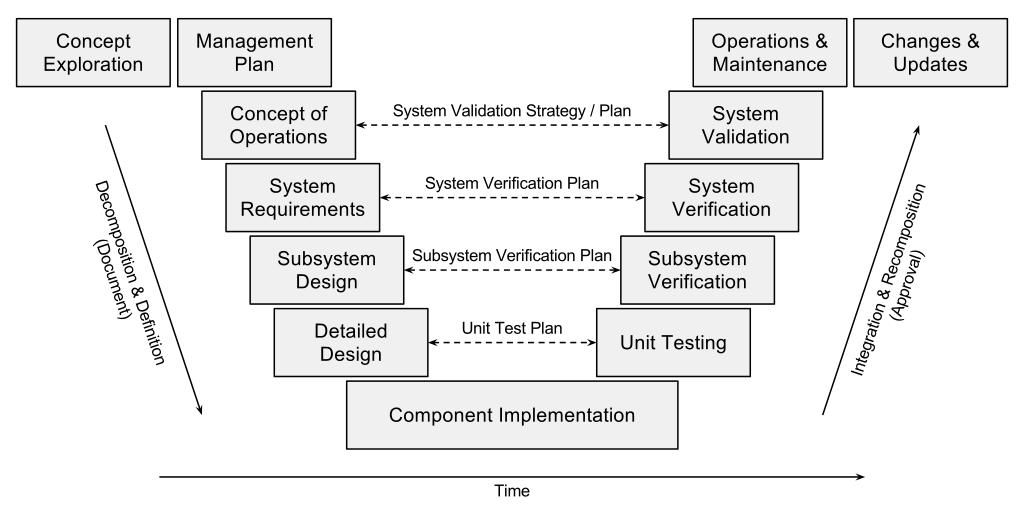
\includegraphics[width=\textwidth]{Thesis/Literature_Review/Lit Review Figures/sysengvee.png}
    \caption{Systems Engineering "Vee"}
    \label{fig:Systems Engineering "Vee"}
\end{figure}

Traditionally, the Systems Engineering process used a "document-based" approach, where documents are the primary artifacts available to stakeholders \citep{Delligatti}. These documents include requirement and traceability matrices, interface documents, concept of operation documents, and other unique documents in a wide variety of formats, such as Microsoft Excel sheets, Adobe PDF documents, Microsoft PowerPoint presentations, and digital drawings. As systems become more complex, the traditional document-based approach becomes challenging to maintain. Each document is manually generated, so file management and version control becomes problematic. It is difficult to know for sure if something is the current version or if it has been subsequently updated but located on some other file system or storage drive. Furthermore, any changes in one document, drawing, etc., must be also made in any other document that uses that same item. This system is prone to errors, inconsistencies, and difficulties maintaining an accurate representation of the entire system. MBSE provides a solution to these increasingly relevant problems. In MBSE, a system model represents the system and any information needed for documents can be found within this model. The model also makes it much easier to maintain consistency. If the modeler updates a component or interface in one area, it will be updated throughout the system as appropriate. Traditionally, acquisition programs reviews will still require paper documents, but the necessary information for those can still be found within the system model during the transition from documents to system models. 

MBSE requires a modeling language, a modeling method, and a modeling tool \citep{Delligatti}. In this paper, those are respectively the \abbreviationFull[Systems Modeling Language]{SysML}, the \abbreviationFull[Object-Oriented Systems Engineering Method]{OOSEM}, and the Cameo Systems Modeler tool.  

SysML is a standard modeling language, which added systems engineering functionality to the \abbreviationFull[Unified Modeling Language]{UML} that has been used extensively in Software Engineering for decades \citep{Delligatti}. SysML provides a language, or the definitions and notations for nine different diagram types to describe a complex system, many of which will be used in this Reference Architecture. SysML is expressed graphically through those diagrams, listed in Figure \ref{fig:SysML Taxonomy} to show various system viewpoints. For example, a \abbreviationFull[Block Definition Diagram]{bdd} expresses system structure, and an Activity Diagram can show specific system activities. Within "blocks", further detail can be expressed on an \abbreviationFull[Internal Block Diagram]{ibd}. Further explanations will accompany their respective diagrams in Chapter \ref{analysisandresults}, but for now, it's important to know that SysML provides the language and is built into the modeling tool, described later in this chapter. 

The modeling method is the specific methodology used to ensure important design tasks have been accomplished and provides the general guidance, processes, or steps for the system design. This paper will focus on OOSEM, but there are other popular methods, such as the \abbreviationFull[Weilkiens System Modeling]{SYSMOD} method and the IBM Telelogic Harmony-SE method \citep{Delligatti}. 

\begin{figure}[!h]
    \centering
    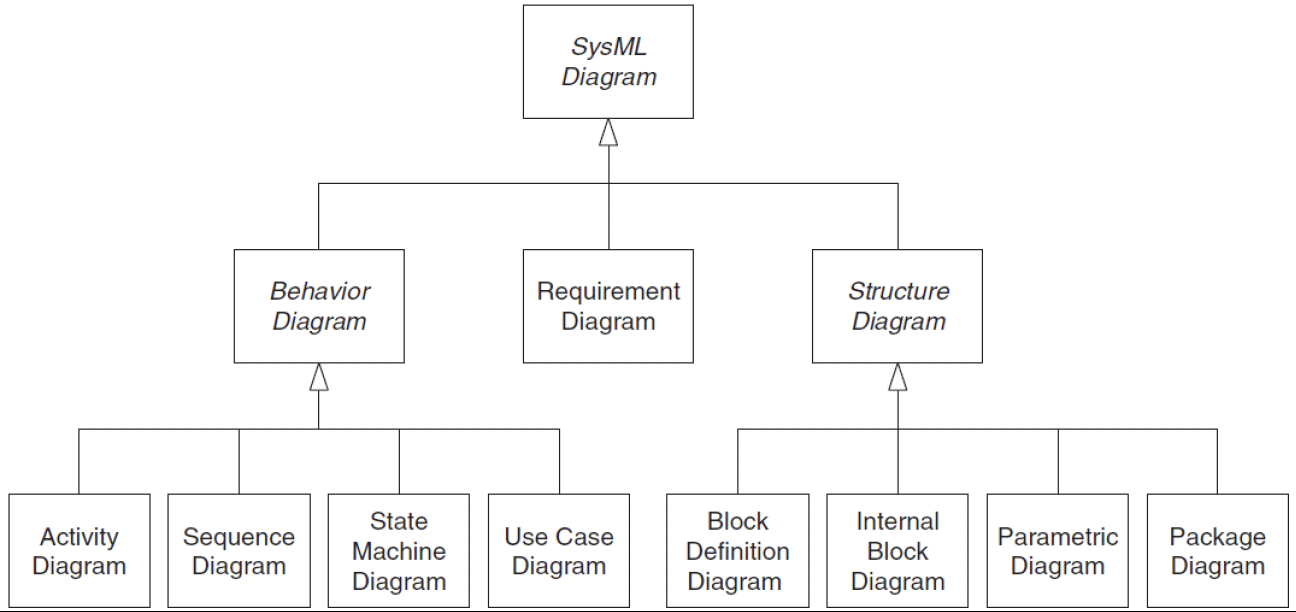
\includegraphics[width=5in]{Thesis/Literature_Review/Lit Review Figures/sysML taxonomy.png}
    \caption{SysML Taxonomy}
    \label{fig:SysML Taxonomy}
\end{figure}

OOSEM uses SysML in a top-down, model-based approach that leverages object-oriented concepts with traditional systems engineering methods to architect more flexible and extensible systems and can evolve with technology and changing requirements \citep{Estefan2008}. OOSEM was developed in part by Lockheed Martin Corporation as a method to capture and analyze requirements of complex systems, integrate with object-oriented software and hardware, and support system-level reuse and design evolution \citep{INCOSEhandbook}.

The primary OOSEM activities are similar to those in the traditional "Systems Engineering Vee" as described previously and are accomplished in an iterative fashion \citep{OMGwiki}. Similarly to the "Vee" method, the traditional technical management processes are still applied at each iteration.

The primary OOSEM steps are as follows:
\begin{enumerate}
\item{\textbf{Analyze Stakeholder Needs:} Capture the "as-is" system and mission enterprise and identify gaps or issues. The "as-is" depiction helps develop the "to-be" system, and the gaps or issues can help drive mission requirements for the new system. OOSEM frequently uses measures of effectiveness for the primary mission objectives identified in this step.}
\item{\textbf{Define System Requirements:} Once the "as-is" system is defined and produces Mission Requirements, the system is modeled as a "black box" in a Mission Enterprise model. For example, instead of going deep into subsystem-level detail on a CubeSat, the entire CubeSat will be a "black box" that interacts with ground stations, other satellites, and the environment. This "black box" model allows for system-level activity diagrams and use cases to show how the "to-be" system will support the mission enterprise. This step helps derive system-level functional, performance, and interface requirements.}
\item{\textbf{Define Logical Architecture:} A "logical" architecture is created that captures key functions in logical blocks, allowing for specific components to be chosen later in place of the logical depiction.}
\item{\textbf{Synthesize Candidate Allocated Architectures:} From the logical architecture, create potential physical instantiations using value properties and selected components. Each component at this stage is then traced to system requirements in table or matrix form.}
\item{\textbf{Optimize and Evaluate Alternatives:} Trade studies or other analysis is conducted at this step among the candidate architectures. Parametric diagrams within the model or integrating other tools can simulate system performance with the chosen components so alternative solutions can be compared.}
\item{\textbf{Validate and Verify System:} Once a candidate architecture has been chosen from the alternatives, the system needs to be validated and verified to ensure the requirements are being met and that stakeholder needs are satisfied. This step uses inspection, demonstration, analysis, and test activities to validate and verify the system.}
\end{enumerate}

Finally, the modeling tool is how the language and method get put together. The modeling tool is a critical piece of software that builds an underlying model of the system that can be used to display many different viewpoints or diagrams, depending on what is needed. The system model in a modeling tool is comprised of model elements and relationships between those elements, and from those, diagrams can be generated. When the source element or relationship is modified or deleted, that change gets carried out throughout the entire model, in any and all diagrams those elements or relationships appeared. This paper will focus on the Cameo Systems Modeler tool from No Magic Inc., but the process is tool-agnostic. Other tools are available on the market to accomplish the same goals with different user interfaces and feature sets. The Cameo Systems Modeler tool will be shown in model screenshots throughout this thesis. 
